% This file was created with tikzplotlib v0.10.1.post5.
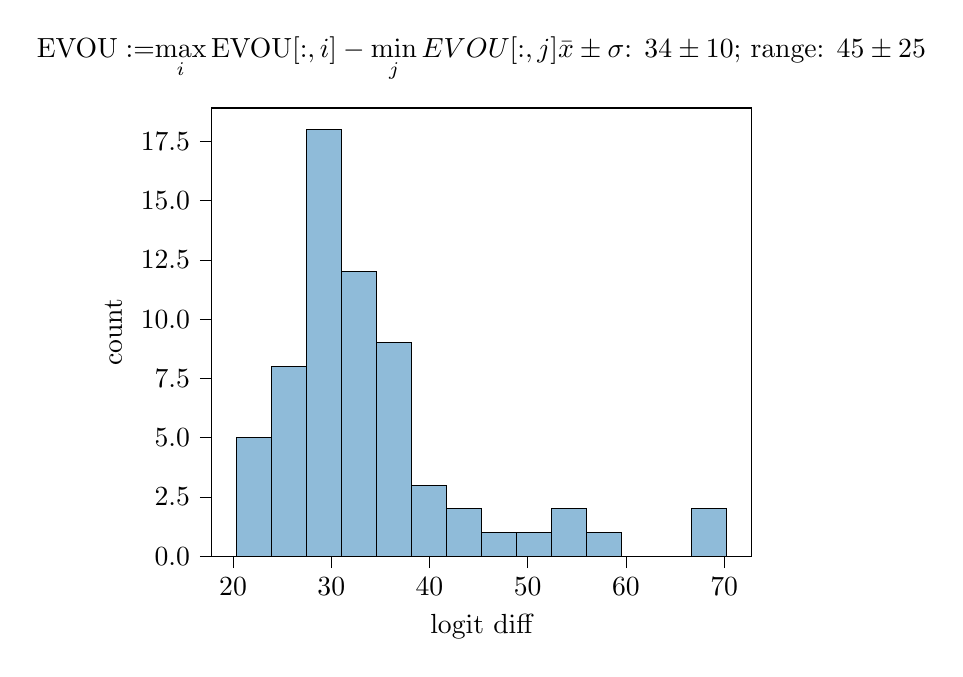
\begin{tikzpicture}

\definecolor{darkgray176}{RGB}{176,176,176}
\definecolor{steelblue31119180}{RGB}{31,119,180}

\begin{axis}[
tick align=outside,
tick pos=left,
title={\(\displaystyle \mathrm{EVOU} := \WE \WV \WO\WU \)\\
\(\displaystyle \max_i\mathrm{EVOU}[:,i] - \min_jEVOU[:,j]\)\\
\(\displaystyle \bar{x}\pm\sigma\): \(\displaystyle 34 \pm 10\); range: \(\displaystyle 45 \pm 25\)},
x grid style={darkgray176},
xlabel={logit diff},
xmin=17.8152199745178, xmax=72.7508906364441,
xtick style={color=black},
xtick={10,20,30,40,50,60,70,80},
xticklabels={
  \(\displaystyle {10}\),
  \(\displaystyle {20}\),
  \(\displaystyle {30}\),
  \(\displaystyle {40}\),
  \(\displaystyle {50}\),
  \(\displaystyle {60}\),
  \(\displaystyle {70}\),
  \(\displaystyle {80}\)
},
y grid style={darkgray176},
ylabel={count},
ymin=0, ymax=18.9,
ytick style={color=black},
ytick={0,2.5,5,7.5,10,12.5,15,17.5,20},
yticklabels={
  \(\displaystyle {0.0}\),
  \(\displaystyle {2.5}\),
  \(\displaystyle {5.0}\),
  \(\displaystyle {7.5}\),
  \(\displaystyle {10.0}\),
  \(\displaystyle {12.5}\),
  \(\displaystyle {15.0}\),
  \(\displaystyle {17.5}\),
  \(\displaystyle {20.0}\)
}
]
\draw[draw=black,fill=steelblue31119180,fill opacity=0.5] (axis cs:20.3122959136963,0) rectangle (axis cs:23.8795472553798,5);
\draw[draw=black,fill=steelblue31119180,fill opacity=0.5] (axis cs:23.8795472553798,0) rectangle (axis cs:27.4467985970633,8);
\draw[draw=black,fill=steelblue31119180,fill opacity=0.5] (axis cs:27.4467985970633,0) rectangle (axis cs:31.0140499387469,18);
\draw[draw=black,fill=steelblue31119180,fill opacity=0.5] (axis cs:31.0140499387469,0) rectangle (axis cs:34.5813012804304,12);
\draw[draw=black,fill=steelblue31119180,fill opacity=0.5] (axis cs:34.5813012804304,0) rectangle (axis cs:38.1485526221139,9);
\draw[draw=black,fill=steelblue31119180,fill opacity=0.5] (axis cs:38.1485526221139,0) rectangle (axis cs:41.7158039637974,3);
\draw[draw=black,fill=steelblue31119180,fill opacity=0.5] (axis cs:41.7158039637974,0) rectangle (axis cs:45.283055305481,2);
\draw[draw=black,fill=steelblue31119180,fill opacity=0.5] (axis cs:45.283055305481,0) rectangle (axis cs:48.8503066471645,1);
\draw[draw=black,fill=steelblue31119180,fill opacity=0.5] (axis cs:48.8503066471645,0) rectangle (axis cs:52.417557988848,1);
\draw[draw=black,fill=steelblue31119180,fill opacity=0.5] (axis cs:52.417557988848,0) rectangle (axis cs:55.9848093305315,2);
\draw[draw=black,fill=steelblue31119180,fill opacity=0.5] (axis cs:55.9848093305315,0) rectangle (axis cs:59.5520606722151,1);
\draw[draw=black,fill=steelblue31119180,fill opacity=0.5] (axis cs:59.552060672215,0) rectangle (axis cs:63.1193120138986,0);
\draw[draw=black,fill=steelblue31119180,fill opacity=0.5] (axis cs:63.1193120138986,0) rectangle (axis cs:66.6865633555821,0);
\draw[draw=black,fill=steelblue31119180,fill opacity=0.5] (axis cs:66.6865633555821,0) rectangle (axis cs:70.2538146972656,2);
\end{axis}

\end{tikzpicture}
